%!TEX root = pir-main-new.tex

\section{Main Constructions}
In this section, we present our main constructions. %In Section~\ref{sec:main}
We present our construction of preprocessing PIR schemes that have
sublinear online computation and communication, and follows from only one-way
functions. 
The constructions can run in both of the two-server setting and the single-server setting, with different preprocessing implementations.
%In Section~\labelcref{sec:polylog}, we present a single server
We will first introduce a simpler scheme that achieves $O(\lambda
n^{1/4}\polylog (\kappa))$ online communication cost in~\Cref{sec:two-server} and~\Cref{sec:single-server}. Then,
we will introduce an optimized, more involved scheme that achieves $O(\lambda
n^{1/4})$ online communication cost in~\Cref{sec:optimized}, removing the
$\polylog (\kappa)$ factor.

%\subsection{Sublinear Preprocessing PIR without Public Key Cryptography}
\label{sec:nquarter}
\label{sec:main}
\label{sec:main-scheme}

\subsection{Starting point: $\Piano$~\cite{piano}, a PIR scheme with $\sqrt{n}$ online communication cost} 

We start by recalling the
high level ideas involved in a the $\Piano$ construction that supports a single
query with $O(\sqrt{n})$ online communication.

Let the database be $\DB$  of size $n$, indexed by $0,\ldots,n-1$. Divide the
database into $\sqrt{n}$ chunks, where chunk $i$ contains the indices of
$\{i\sqrt{n},i\sqrt{n}+1,\dots,(i+1)\sqrt{n}-1\}$. We define
$\chunk(x)=\left\lfloor \frac{x}{\sqrt{n}}\right\rfloor$. During the
preprocessing phase, the client generates many random sets $S_1,\dots,S_{M_1}$.
Each random set will contain exactly one random index from each chunk and have
$\sqrt{n}$ indices. The client stores the parities for those sets . For example,
$p_1=\xor_{x\in S_1}\DB[x]$. Moreover, the client stores, for each chunk,
polylogarithmically many pairs of random indices and their corresponding
database values. We call these index-value pairs as replacement pairs.
For now, we just assume the client can run the preprocessing phase in a server-oblivious fashion. 
We defer the details of implementing preprocessing phase to~\Cref{sec:two-server} and~\Cref{sec:single-server}.

In order to make an online query on the index $x$, the client first finds a set
$S_i$ that $x\in S_i$. The client only needs to know the parity of $S_i/\{x\}$
because $\DB[x]=p_i \xor\left(\xor_{x'\in S_i/\{x\}}\DB[x']\right)$, and $p_i$
is known. To achieve this, the client lists out all $\sqrt{n}$ indices in $S_i$,
replaces $x$ with an unconsumed replacement index, say $y$, from the same chunk
of $x$ and sends these $\sqrt{n}$ indices to the server. The server computes the
parities of these indices and returns a bit $\beta$ to the client, which only
takes $O(\sqrt{n})$ time. Now the client knows $\beta=\left(\xor_{x'\in
S_i/\{x\}}\DB[x']\right)\xor \DB[y]$. Notice that $\DB[y]$ is known to the
client by preprocessing, so the client can compute the parity of $S_i/\{x\}$,
and therefore $\DB[x]$.

It is not difficult to prove that if the preprocessing is oblivious to the online server, the
server simply sees a random set that contains $x$ and then $x$ is replaced with
a random index within the same chunk. This set is identically distributed as a
uniformly random set. %Moreover, the during the preprocessing, the client reads
%the database in a streaming fashion, reading a chunk at a time to compute all
%the parities it needs to store. Hence, the preprocessing is indeed oblivious to
%the server. 
Therefore, the scheme is private.

To compress the local storage, the client can use a pseudorandom function
$\PRF:\{0,1\}^\lambda \times \{0,\dots,\sqrt{n}-1\} \to \{0,\dots,\sqrt{n}-1\}$
and represent a set with a $\lambda$-bit key $\sk$. Define $\Set(\sk)$ as
follows: for $j\in \{0,1,\ldots,\sqrt{n}-1\}$, the $j$-th element of
$\Set(\sk)$, denoted as $\Set(\sk)[j]=\PRF(\sk, j) + j\sqrt{n}$. In other words,
we use the PRF to expand the keys to $\sqrt{n}$ \emph{offsets} and the $j$-th
offset is the offset of the random index inside the $j$-th chunk. The client
only needs $\widetilde{O}(\sqrt{n})$ sets, so the client storage cost is
$\widetilde{O}_\lambda(\sqrt{n})$. 
%Also in the actual protocol, the client sends
%the offsets of each chunk, instead of sending over the set. 

\subsection{Reducing online communication to $\widetilde{O}_\lambda(n^{1/4})$
bits}
%Notice that $\Piano$ has to expand the set and send all $\sqrt{n}$ indices to
%the server where there are exactly one replaced index. This replacement trick
%is where the challenge of optimizing the communication : it seems like without 
Towards our goal of reducing communication, we will introduce the notion of {\bf
superblocks}. We group $n^{1/4}$ consecutive chunks into one superblock, so each
superblock contains $n^{3/4}$ indices and there are $n^{1/4}$ superblocks in
total. We define $\superblock(x)=\left\lfloor \frac{x}{n^{3/4}}\right\rfloor$.
Further, we say that the relative location of $\chunk(x)$ in superblock $j$ is
$\chunk(x)-j\cdot n^{1/4}$. 

We propose a new set representation based on a two-layer construction. At a
high-level, given a $\lambda$-bit key, we first expand that key to $n^{1/4}$
\emph{sub-keys} using one PRF. Each sub-key corresponds to one super-block. We
then use another PRF to expand each sub-key to $n^{1/4}$ offsets. The offsets
expanded by a particular sub-key are the offsets of the chunks inside its
corresponding superblock.

Formally, we assume that the $\PRF:\bits^{\lambda}\times \bits^{\frac{\log
n}{2}}\to \bits^{\frac{\log n}{2}}$ is constructed from two different $\PRF$'s
$\PRF_1: \bits^{\lambda}\times \bits^{\frac{\log n}{4}}\to
\bits^{\lambda},\PRF_2:\bits^{\lambda}\times \bits^{\frac{\log n}{4}}\to
\bits^{\frac{\log n}{2}}$ as follows:
\begin{align*}
    \PRF(\sk,x)=\PRF_2(\PRF_1(\sk,\lfloor x / n^{1/4} \rfloor ),x\bmod n^{1/4}).
\end{align*}

\begin{figure*}
    \centering
    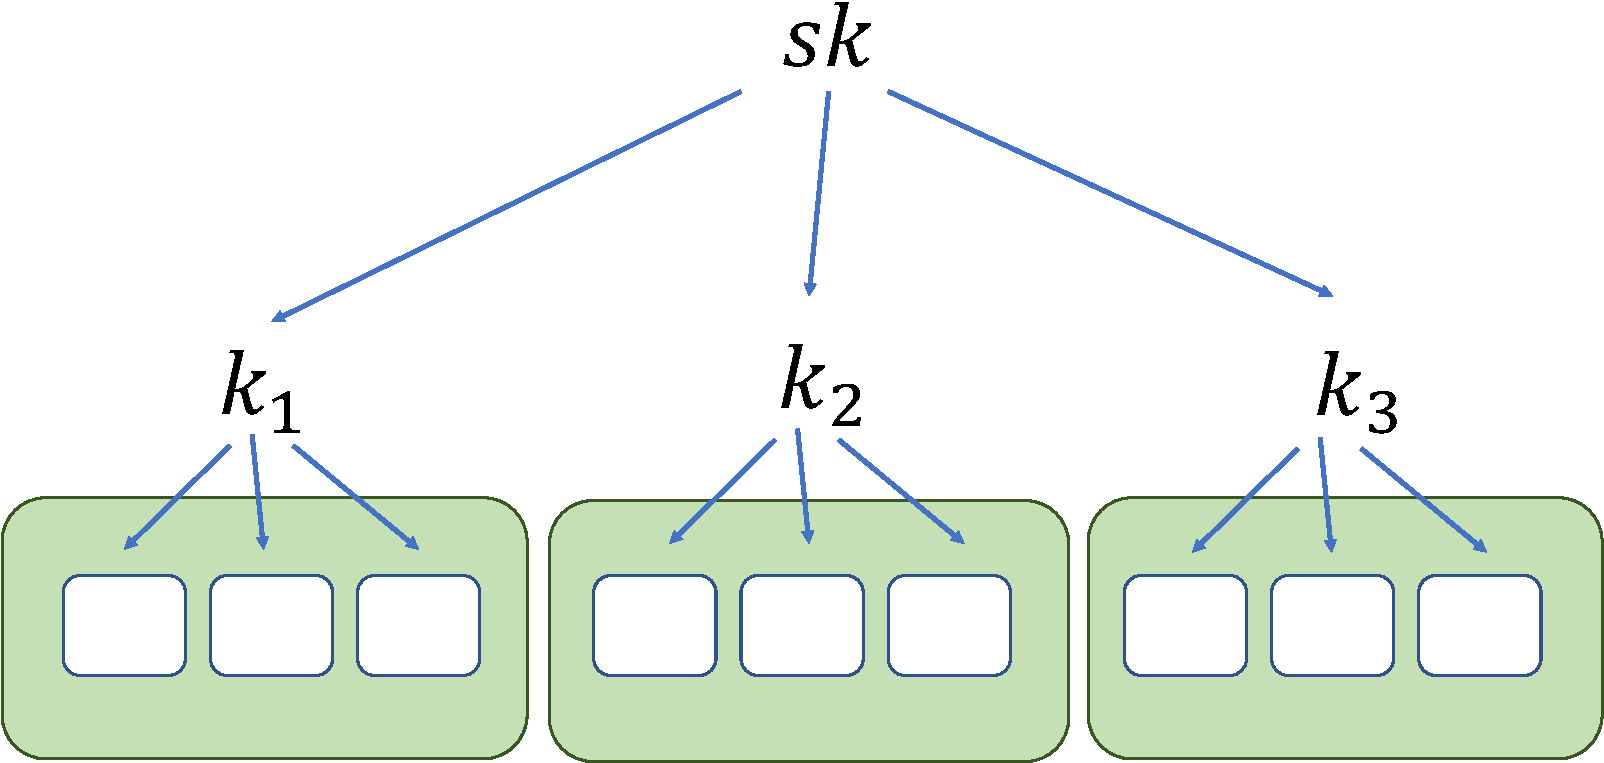
\includegraphics[width=0.6\linewidth]{figs/set-rep.pdf}
    \caption{Two-layer set representation\label{fig:set-rep}. The first layer key expands to $n^{1/4}$ sub-keys. Each sub-key controls a superblock and expands to $n^{1/4}$ offsets. Each offset in a chunk represents an index.}
\end{figure*}

%Here, $x[i:j]$ means the bit string from the $i$-th bit to the $(j-1)$-th bit of $x$'s binary representation.

Again, the high level idea behind the online query is similar: the client finds
a key $\sk$ such that $x\in \Set(\sk)$. The client wants to learn the parity of
$\Set(\sk_i)/\{x\}$. We now present in two-steps below how the two-layer set
representation helps us to reduce the online communication cost to
$\widetilde{O}_\lambda(n^{1/4})$ bits. 

\begin{itemize}
    \item \textit{Step 1: Learning the parities for all superblocks except the
    one containing $x$.}
    
    The client first expands $\sk$ to $n^{1/4}$ sub-keys,
    $k_0,\dots,k_{n^{1/4}-1}$. Now, the client replaces the $\superblock(x)$-th
    sub-key by a uniformly random sub-key $k'\getr\{0,1\}^\lambda$. This ensures
    that from the server's view, these $n^{1/4}$ sub-keys are random after the
    replacement. The client sends these $n^{1/4}$ sub-keys to the server. For
    each superblock $i$, the server will expand the $i$-th sub-key to $n^{1/4}$
    offsets and consider them as the offsets for the $n^{1/4}$ chunks in the
    superblock $i$. The server computes the parity for the $n^{1/4}$ indices
    corresponding to the offsets. Denote the parity as $\alpha_i$. The server
    returns $(\alpha_0,\dots,\alpha_{n^{1/4}-1})$ to the client. Then, except
    $\alpha_{\superblock(x)}$, all other $\alpha$ are the correct parities for
    their corresponding superblocks. The client can simply compute the xor-sum
    of those $n^{1/4}-1$ superblocks.

    \item \textit{Step 2: Learning the parity of all other indices in $x$'s
    superblock except $x$.} Now, the client expands $k_{\superblock(x)}$ to
    $n^{1/4}$ offsets, $\delta_0,\dots,\delta_{n^{1/4}-1}$. Notice that in the
    relative location of $x$'s chunk, the offset will be $x \mod \sqrt{n}$.
    Recall that the client already preprocessed polylogarithmic random
    replacement, i.e., index-value pairs in each chunk. Assume the first
    unconsumed replacement index in $x$'s chunk is $y$. The client simply
    replaces $x$'s offset to $y$'s offset and sends those $n^{1/4}$ offsets to
    the server. This ensures that from the server's view, these $n^{1/4}$
    offsets are random after the replacement. Upon receiving those offsets, the
    server does not know which superblock they correspond to. However, the
    server can just enumerate all $n^{1/4}$ possible cases: for
    $i\in\{0,\dots,n^{1/4}\}$, the server considers those $n^{1/4}$ offsets are
    the offsets of those items in the $n^{1/4}$ chunks of the $i$-th superblock,
    and computes the corresponding parity $\beta_i$. The server returns
    $(\beta_0,\dots,\beta_{n^{1/4}-1})$ to the client. The client knows that
    $\beta_{\superblock(x)}$ is the correct parity for $x$'s superblock, except
    that the index $x$ is replaced with $y$. After removing the influence of $y$
    (the client already knows $\DB[y]$), it knows the parity of those indices
    inside $x$'s superblock except $x$.

\end{itemize}

Finally, the client can learn the parity of $ \Set(\sk)/\{x\}$ by xoring the answers from step 1 and 2. Then the client can derive $\DB[x]$.
Notice that in this algorithm, the client sends $n^{1/4}$ sub-keys and $n^{1/4}$ offsets to the server, and the server returns $2n^{1/4}$ parities (bits) to the client. 
So the communication cost is $O_\lambda(n^{1/4})$.
Also, the server's computation time in both steps is simply $O_\lambda(\sqrt{n})$ without any further optimization.
We present the pseudocode for the single query algorithm in~\Cref{fig:single-query}.

\begin{figure}
    \centering
    \begin{subfigure}[b,labelformat=empty]{0.48\textwidth}
        \centering
        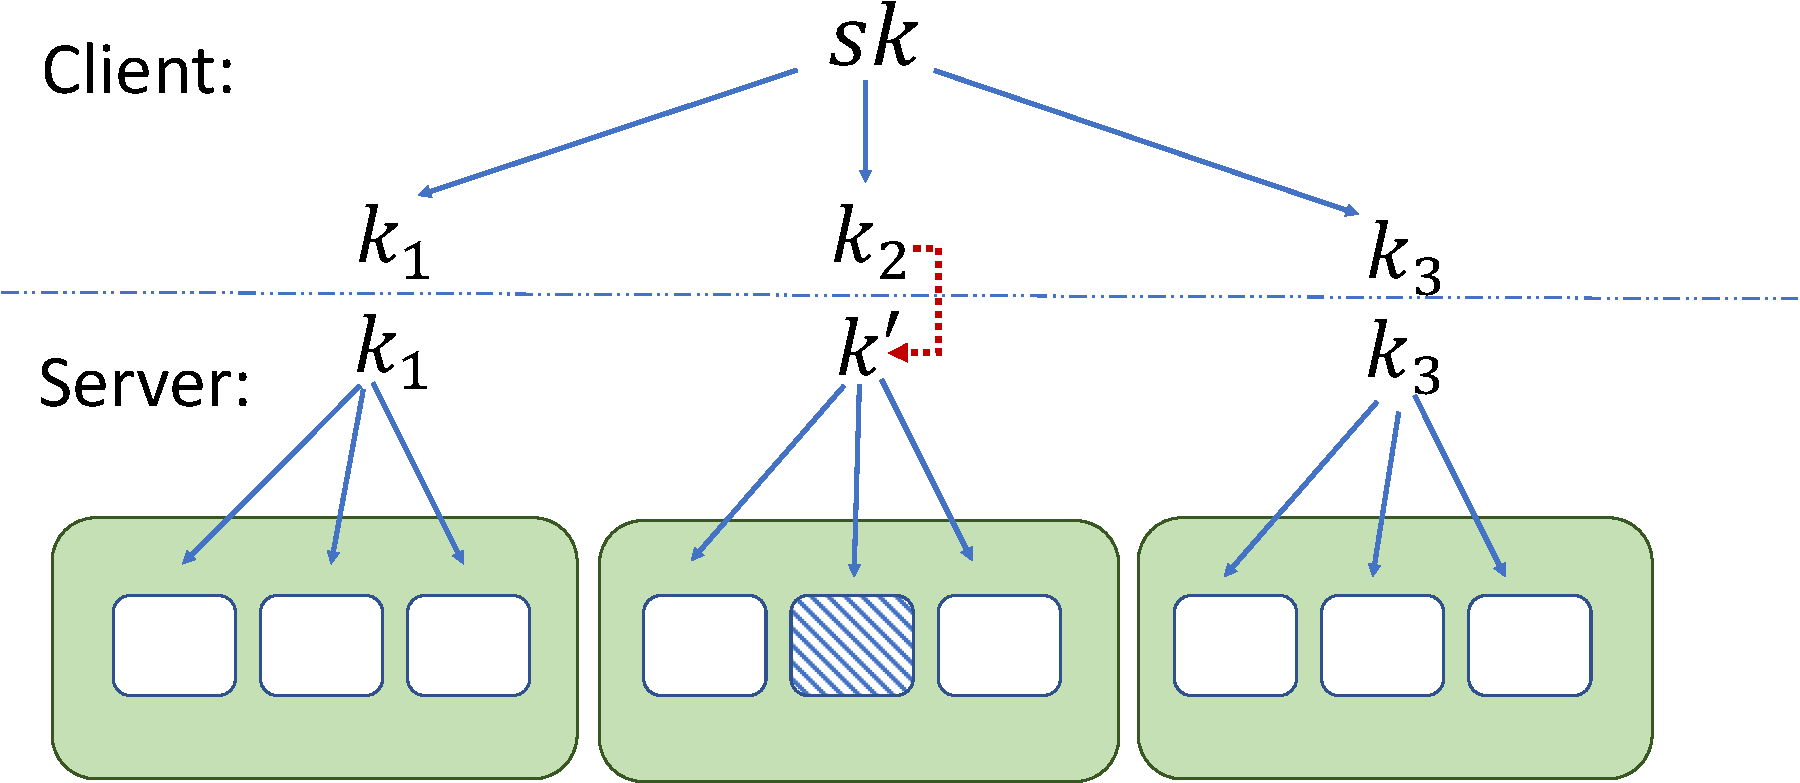
\includegraphics[width=\textwidth]{figs/step1.pdf}
        \caption*{Step 1: The client expands the main key to $n^{1/4}$ sub-keys and replaces the one that controls $x$'s superblock to a uniformly random one. The server returns $n^{1/4}$ parities for those $n^{1/4}$ superblocks.}
        % \label{fig:step1}
    \end{subfigure}
    \hfill
    \begin{subfigure}[b,labelformat=empty]{0.48\textwidth}
        \centering
        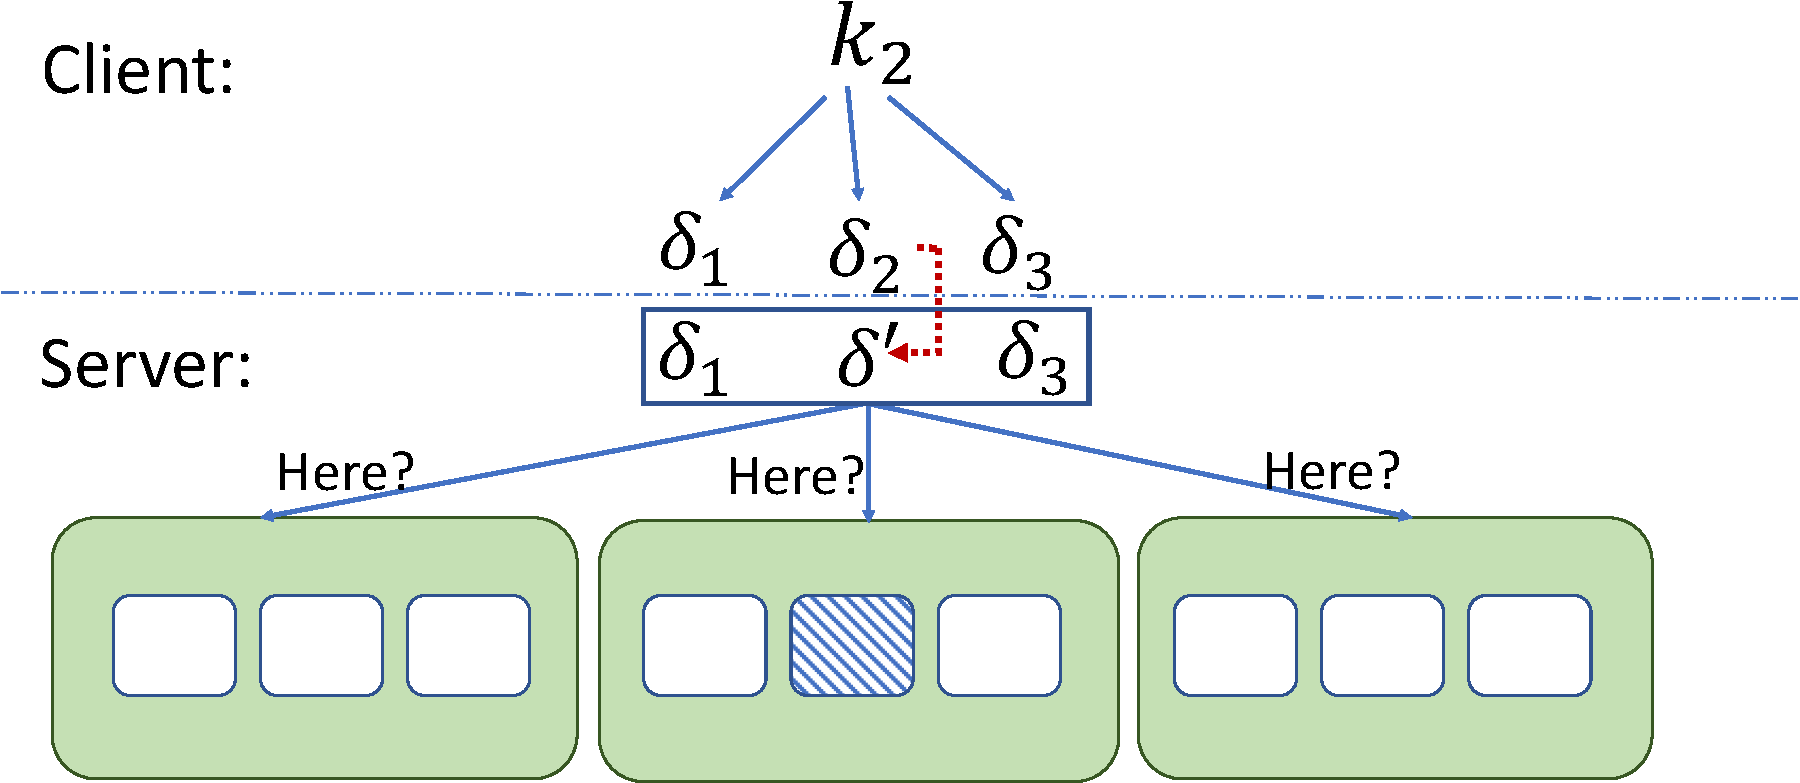
\includegraphics[width=\textwidth]{figs/step2.pdf}
        \caption*{Step 2: The client expands the sub-key to $n^{1/4}$ offsets and replaces the offset of $x$ to a random one. The server puts those offsets into every superblock. Returns $n^{1/4}$ corresponding parities. }
        % \label{fig:step2}
    \end{subfigure}
    \caption{Demonstration of the single-query algorithm assuming the query is in the middle chunk. The server does not know where the query is because the replacing operations are oblivious.}
    \label{fig:algo}
\end{figure}

%The main idea in our new construction is instead of sending over the offsets of $\sqrt{n}$ values, the client will send over $n^{1/4}$ ``sub-keys'' and $n^{1/4}$ offsets, thereby reducing the communication. The sub-keys will be $\lambda$ bits long and will correspond to a superblock. Further, a sub-key will be sufficient to compute all the offsets of a chunk in a superblock. 

%In order to read the value at index $x$, the client will compute the $n^{1/4}$ sub-keys for all the chunks, and compute all the offsets only for the chunks in same superblock as $x$ is in. The client then sends over {\bf 1)} all the sub-keys, except the one for the superblock of $x$, replacing it with a random sub-key {\bf 2)} all the offsets for the chunks in the superblock of $x$, except the offset for $\chunk(x)$, replacing it with the offset of a random element $r$ which is in $\chunk(x)$, such that $\DB[r]$ was stored during preprocessing.

%We need to specify how these sub-keys for the superblocks are computed given the $\PRF$ key. Here, we utilize the underlying structure of the $\PRF$ . We assume that the $\PRF:\bits^{\lambda}\times \bits^{\frac{\log n}{2}}\to \bits^{\frac{\log n}{2}}$ is constructed from two different $\PRF$'s $\PRF_1: \bits^{\lambda}\times \bits^{\frac{\log n}{4}}\to \bits^{\lambda},\PRF_2:\bits^{\lambda}\times \bits^{\frac{\log n}{4}}\to \bits^{\frac{\log n}{2}}$ as follows:
%\begin{align*}
%    \PRF(\sk,x)=\PRF_2(\PRF_1(\sk,x[0]),x[1])\;,
%\end{align*}
%where $x[0],x[1]$ denote the first $\frac{\log n}{4}$ and last $\frac{\log n}{4}$ bits of $x$ respectively. The GGM construction~\cite{GGM86} in particular can be viewed to be of this form.

%Given $\sk$, the sub-key for superblock $i$ is $k_i=\PRF_1(\sk,i)$ for $i\in \{0,1,\ldots,n^{1/4}-1\}$. Note that all the offsets for chunk $i$ can be computed using $k_i$. As specified above, the client sends over $n^{1/4}$ different sub-keys and $n^{1/4}$ different offsets to the server. Label the sub-keys received by the server as $k_0',k_1',\ldots,k_{n^{1/4}-1}'$ and label the offsets as $\delta_0',\delta_1',\ldots,\delta_{n^{1/4}-1}'$.

% \heading{Superblocks, sub-keys and the low bandwidth construction.} Let $x_0\in \bits^{\frac{\log n}{2}}$. Observe that, because of the property of $\PRF$, if the client provides the evaluation of $\PRF_1(\sk,x_0)$, the server can compute $\PRF(\sk,x_0\concat x_1)=\PRF_2(\PRF_1(\sk,x_0),x_1)$ for any $x_1\in \bits^{\frac{\log n}{2}}$. We use this observation to compress the online bandwidth.
% If the client wants to read the location $x$, and $\sk$ is a hint such that $x\in\Set(\sk)$, for all $y\in \{0,1,\ldots,n^{1/4}-1\}$, the client compute $\PRF_1(\sk,y)$. Let these values be $k_0,k_1,\ldots,k_{n^{1/4}-1}$ -- we refer to them as ``sub-keys''. 

% We introduce a new terminology: for every $x\in \{0,\ldots,{n}-1\}$ we say that $x$ is in the ``superblock" $j$ if $\lfloor x/n^{1/4}\rfloor = j$. Further, we say that the relative location of $\chunk(x)$ in superblock $j$ is $\chunk(x)-j\cdot n^{1/4}$. 

% We also refer to $k_j$ as the sub-key for that superblock. Let $b^*=\superblock(x)$ and $d^*$ be the relative location of $\chunk(x)$ in $\superblock(x)$, i.e. $d^*=\chunk(x)-\superblock(x)\cdot n^{1/4}$. Let $\delta_i=\PRF_2(k_{b^*},i)$ for $i\in \{0,1,\ldots,n^{1/4}-1\}$.
% Let $k'$ be a randomly sampled sub-key and let $r$ be a random value in $\{0,\ldots,n-1\}$ such that $\DB[r]$ such that $\chunk(r)=\chunk(x)$ had been read and stored by the client during the preprocessing. Let $\delta=r \text{ mod }\sqrt{n}$. The client sends over the following to the server:
% \begin{itemize}
%     \item the subkeys $k_0,\ldots,k_{n^{1/4}-1}$ \emph{except} $k_{b^*}$, replacing it with $k'$, 
%     \item the offsets $\delta_0,\ldots,\delta_{n^{1/4}-1}$ \emph{except} $\delta_{d^*}$, replacing it with $\delta'$.
% \end{itemize}

%For each $b\in \{0,\ldots,n^{1/4}-1\}$, the server computes the offsets for the $b$-th sub-key $k_b$, i.e. computes $\PRF_2(k_b',y)$ for each $y\in \{0,1,\ldots,n^{1/4}-1\}$. Assuming that this $b$-th sub-key is the sub-key for the $b$-th superblock (this assumption is correct except for the superblock $x$ is in), it computes the xor-sum of all the database entries indexed by the values in the superblock. Call this xor-sums $\alpha_b$. Next for $b\in  \{0,\ldots,n^{1/4}-1\}$, the server assumes that the offsets were of the $b$-th superblock and computes the xor-sum of the super-block accordingly (this assumption in contrast is \emph{only} correct for the superblock $x$ is in). Call the xor-sums $\beta_b$. The server sends over all the $\alpha_b$'s and $\beta_b$'s for $b\in  \{0,\ldots,n^{1/4}-1\}$ to the client.

\begin{figure}[p]
    
    \begin{minipage}{\textwidth}
        \begin{mdframed}
            \label{alg:one-query}
            \begin{center}
                {\bf Query Protocol for a Single Query $x$: $\SingleQuery(x,
                \sk, p_{\sk}, r, p_r)$.
                    %\andy{Is it not $O(\sqrt{n})$?}
                }
            \end{center}
            
            \parhead{Client's input:}
            %Suppose the client has the following inputs:
            \begin{itemize}
                \item A master PRF key $\sk$ assuming $x\in \Set(\sk)$;
                \item The parity of $\Set(\sk)$ is assumed to be $p_{\sk}$;
                \item A random index $r$ in $x$'s chunk such that the  $\DB[r]$
                is assumed to be $p_r$.
            \end{itemize}
            
            %\parhead{Suppose the client has a hint $$} When a query $x \in \{0,
            %1, \ldots, n-1\}$ arrives, \Client performs the following: 
            \begin{enumerate}[leftmargin=5mm,itemsep=1pt]
                \item 
                {\bf Step 1: (Client)}

                \begin{enumerate}[leftmargin=5mm,itemsep=1pt]
                        
                        \item Let $b^*={\sf superblock}(x)=\lfloor x/n^{3/4}
                        \rfloor, c^* = {\sf chunk}(x)=\lfloor x/n^{1/2}
                        \rfloor$. Let $d^*=\chunk(x)\mod n^{1/4}$ be the
                        relative chunk location of $x$ in the superblock. 
                        

                        \item Expand $\sk$ to $n^{1/4}$ sub-keys $k_{
                        0},\dots,k_{n^{1/4}-1}$ where $k_{b}=\PRF_1(\sk, b)$ for
                        all $b$.
                    
                        \item Expand the $b^*$-th sub-keys to $n^{1/4}$ offsets
                        $\delta_{0},\dots,\delta_{n^{1/4}-1}$ where
                        $\delta_{\ell}=\PRF_2(k_{b^*}, \ell)$.
                        
                        \item Sample a random sub-key $k'\getr\{0,1\}^\lambda$
                        and denote $\delta'=r\mod \sqrt{n}$.
                        \item Send the following tuples to the server:
                        \begin{align*}
                            (k_{0},\dots,k_{b^*-1}, k',k_{b^*+1},\dots,k_{n^{1/4}-1}) \\
                            (\delta_{0},\dots,\delta_{d^*-1},\delta' ,\delta_{d^*+1},\dots,\delta_{n^{1/4}-1})
                        \end{align*}
                    
                \end{enumerate}
                
                \newpage
                
                \item 
                {\bf Query Step 2: (Server)}
                
                Upon receving the tuples $(k'_0,\dots,k'_{n^{1/4}-1})$,
                $(\delta'_0,\dots,\delta'_{n^{1/4}-1})$: 
                \begin{enumerate}
                    \item For $b\in \{0,\dots,n^{1/4}-1\}$:
                    \begin{enumerate}
                        \item Expand $k'_b$ to $n^{1/4}$ offsets and consider
                        them being the corresponding index offsets in chunk $\{b
                        \cdot n^{1/4}, \ldots, (b + 1)\cdot n^{1/4} -1\}$.
                        Compute the xor-sum of the database values for those
                        indices as 
                        \[
                        \alpha_b=\xor_{c\in \{0,\dots,n^{1/4}-1\}} \DB[(c + bn^{1/4})\sqrt{n} + \PRF_2(k'_b, c)].
                        \]
                        \item Consider $(\delta'_0,\dots,\delta'_{j,n^{1/4}-1})$
                        as the corresponding index offsets in chunk $\{b \cdot
                        n^{1/4}, \ldots, (b + 1)\cdot n^{1/4} -1\}$. Compute the
                        xor-sum of the database values for those indices as 
                        \[
                        \beta_b=\xor_{c\in \{0,\dots,n^{1/4}-1\}} \DB[(c + bn^{1/4})\sqrt{n} + \delta_c].
                        \]
                    \end{enumerate}
                    
                    \item Return $(\alpha_0,\dots,\alpha_{n^{1/4}-1}),
                    (\beta_0,\dots,\beta_{n^{1/4}-1})$ to the client.
                \end{enumerate}
                
                
                \item 
               {\bf Step 3: (Client)}
               
               Upon receiving $(\alpha_0,\dots,\alpha_{n^{1/4}-1}),
               (\beta_0,\dots,\beta_{n^{1/4}-1})$:
                \begin{itemize}[leftmargin=5mm,itemsep=1pt]
                    \item 
                    The xor-sum of the items in $\Set(\sk)$ except those in the
                    superblock of $x$ is
                    $\alpha=\sum_{b\in\{0,\dots,n^{1/4}-1\},b\ne b^*}\alpha_b$.
                    
                    \item The xor-sum of the items in the superblock of $x$
                    except $x$ is $\beta=\beta_{b^*}\xor p_r$.
                    
                    \item Then, the value of $x$ is
                    $\DB[x]=p_\sk\xor\alpha\xor\beta$.
                \end{itemize}
            \end{enumerate}
        \end{mdframed}
    \end{minipage}
    \caption{Query Protocol for a single query that reduces communication to
    $O(n^{1/4})$. This is used as a sub-routine in the sublinear single server
    PIR scheme presented in Section~\labelcref{sec:nquarter}.}
    \label{fig:single-query}
\end{figure}



%Given all the $\alpha_b$'s the client can compute the xor sum of all the values
% indexed by $\Set(\sk)$, except for those in superblock of $x$. From the
% preprocessing the client knows the xor-sum of all the values indexed by
% $\Set(\sk)$ and thereby can compute the xor-sum of all the values indexed by
% the elements in the super-block of $x$. Further, the $\beta_b$'s along with
% the value of $\DB[r]$ for the $r$ client used specify can be used to compute
% $\DB[x]$ from the  xor-sum of all the values indexed by the elements in the
% super-block of $x$. Now, suppose $b^*=\superblock(x)$. Observe that $\alpha=
% \alpha_{b^*}\oplus \sum_{i=0}^{n^{1/4}-1}\alpha_i$ is the xor-sum of the
% database entries indexed by all the values at all the super blocks except
% super-block $b^*$. Further, $\beta=\beta_{b^*}\oplus p_r$ (where $p_r=\DB[r]$,
% the value of the database at $r$, which was stored by the client during
% preprocessing) is the xor-sum of all the entries of the database indexed by
% the values in the super-block $b^*$ except the value indexed by
% $\delta_{d^*}$. If $p_{\sk}$ was the parity of all the bits of the database
% indexed by $\sk$ (that the client stored during preprocessing), it follows
% that $\DB[x]=p_{\sk}\oplus\alpha\oplus \beta$. The client can compute this
% since it has stored $p_r,p_{\sk}$ during preprocessing and received rest of
% the values from the server.


\subsection{Supporting multiple queries in the online phase} 

Thus far, we have
given a new, low-communication protocol that handles only one query. We now want
to make $Q=\sqrt{n}/2$ queries with just one offline phase. For convenience, we
first make some assumptions about the queries without loss of generality, which
are also made in $\Piano$:
\begin{itemize}
    \item \textit{The client does not make repeated queries.} This can be ensured 
    by requiring the client to store a local cache of size $Q$ for caching the
    most recent $Q$ queries. If the client wants a repeated query, it can lookup
    in the cache and make a dummy query.
    
    \item \textit{The queries the client makes are on random indices.} This is a relatively
    strong assumption. However, we argue that it can be made without loss of
    generality and can be done by letting the client and the server agree on a
    pseudorandom permutation (PRP)~\cite{prp1,prp2} upfront and the server can
    permute the database according to the PRP. Another option is let the server
    build the database as a key-value storage and use a cuckoo hash
    table~\cite{cuckoo1,cuckoo2} directly based on a PRF to locate the queries.
    Notice that, in both implementations, the client can still make queries
    adaptively depending on the real query sequnce and the responses, which is
    sufficient for practical usage. Then, as long as the client makes the
    queries independent of the randomness of the PRP/PRF, those queries can be
    considered as uniformly random. This assumption is only needed for the
    correctness.
\end{itemize}

In order to support multiple queries, the key idea that had been used in
$\Piano$ was to ``refresh" the consumed hint by re-programming a fresh hint in a
way that does not change the distribution of the hints. Here, while our high
level goal will be the same, our strategy to do it would be significantly
different. The reason why the approach used in $\Piano$ does not translate here
is because of the following tension. Since in this new protocol we compress
bandwidth by making the client send only \emph{sub-keys} for the superblocks,
re-programming the hint while still having this compression would make
distribution of the client's future messages depend on the current query, which
violates privacy. Therefore, we seem to require newer ideas to avoid this issue.


Our main idea here is that when the client wants to read $x$, they find
\emph{all} the hints $\sk_i$ such that $x\in\Set(\sk_i)$. The client then runs
the single query protocol based on all of these hints\footnote{To ensure privacy, we
will have an probabilistic upper bound on how many queries are made. If the
client does not have that many hints, it pads some dummy queries.}. After these
hints have been consumed, the client needs to generate new hints so that the
distribution of local hints does not change. Here, for each consumed hint, the
client resamples a new key $\sk$ such that $x\in \Set(\sk)$ by rejection
sampling\footnote{The reason why the client cannot replace those hints with a
uniformly random one is that the occurrence of $x$ in the remaining tables are
less likely, and thus skewing the distribution.}. However, this could raise of
problem of ``broken hints'': the client does not know the parity for these newly
generated sets, and thus these new hints are marked as ``broken''. 

The key observation is this: as long as there is at least one non-broken hint
among the chosen hints, then the client can \emph{still} find the right
$\DB[x]$. And we will prove that except with negligible probability, at least
one of the hints for $x$ that the client chooses is not broken. Moreover, the
client only needs to consume the replacement index-value pairs for that single
query based on the one non-broken hint. For every other queries, the client does
not care about the response, so the client just replaces $x$'s offset with a
random offset. Notice that if the client shuffles the order of queries, the
query based on good hint and the queries based on the broken hints are
identically distributed from the server's view. Lastly, we argue that the client needs running time roughly $O(\sqrt{n})$ trials to rejection sample one hint in expectation. This follows since if we sample a random secret key
$\sk$, the probability that $\PRF(\sk,\chunk(x))=x-\chunk(x)\cdot \sqrt{n}$ is
$\Theta(1/\sqrt{n})$ assuming that the $\PRF$ was a random function. There are superlogarithmically many hints that need to be sampled.
This can be done in $\widetilde{O}(\sqrt{n})$ expected
time.

\begin{figure}[p]
    \begin{minipage}{\textwidth}
        \begin{mdframed}
            \label{alg:fullpolyl}
            \begin{center}
                {\bf Single-Server Scheme for $Q=\sqrt{n}/2$ Queries
                    \footnote{For clarity, we present the scheme supporting distinct and random queries. As mentioned before, these restrictions can be removed by applying PRP and local caching.}
                }
            \end{center}
            \parhead{Notation.}
            $\kappa$ denotes a {\it statistical} security parameter, $\lambda$
            denotes a computational security parameter. We use $\alpha(\kappa)$
            to denote an arbitrarily small super-constant function.

           \parhead{Offline preprocessing.} 
            \begin{itemize}[leftmargin=3mm,itemsep=1pt]
                \item 
                \Client samples $M_1=2\sqrt{n}\log \kappa \cdot \alpha(\kappa)$
                master PRF keys denoted $\psk_1, \dots, \psk_{M_1} \in \{0,
                1\}^\lambda$ for the primary table.
                %, where $M_1=\sqrt{n}\log \kappa \cdot \alpha(\kappa)$. , such
                %that $\alpha(n)=\omega(1)$. \elaine{TODO: fix params}
                Initialize the parities $p_1,\dots,p_{M_1}$ to zeros.
                
                %\elaine{TODO: notation inconsistent with earlier text}
                
                \item 
                \Client downloads the whole DB from the server in a streaming
                way: when the client has the $j$-th chunk
                $\DB[j\sqrt{n}:(j+1)\sqrt{n}]$:
                \begin{itemize}
                    \item {\it Update primary table}: for $i \in [M_1]$, let
                    $p_i \get p_i \oplus \DB[\Set(\psk_i)[j]]$.
                    \item {\it Store replacement entries}: sample and store
                    $M_2=3\log \kappa \cdot \alpha(\kappa)$ % \log \kappa\cdot
                    % \alpha(\kappa)$ 
                    tuples of the form $(r, \DB[r])$ where $r$ is a random index
                    from the $j$-th chunk.
                    %independent random indices from $[i\sqrt{n}:(i+1)\sqrt{n}]$
                    %with the associated database values.
                    \item Delete $\DB[j \sqrt{n}:(j +1)\sqrt{n}]$ from the local
                    storage.
                \end{itemize}
                
                \item At this moment, let $T := \{(\psk_i, p_i )\}_{i \in
                [M_1]}$ denote the client's {\it hint table}. Mark all the hints
                as ``good''.
            \end{itemize}
            
            
            
            
            \parhead{Online query for index $x \in \{0, 1, \ldots, n-1\}$.}
            %When a query $x \in \{0, 1, \ldots, n-1\}$ arrives, \Client
            %performs the following: 
            \begin{enumerate}[leftmargin=5mm,itemsep=1pt]
                \item 
                {\bf Query:}
                \begin{enumerate}[leftmargin=5mm,itemsep=1pt]
                    %\item Let %$i^*=\left\lfloor
                    %\frac{x}{\sqrt{n}}\right\rfloor$ be the index of $x$'s
                    %chunk.
                    \item 
                    \Client finds all the matched hints
                    $(\sk_1,p_1),\dots,(\sk_m,p_m)$ in the hint table  such that
                    $x\in \Set(\sk_j)$ for all $j\in[m]$.
                    
                    \item 
                    If there are less than $M_3=6(\ln \kappa \alpha(\kappa))^2$
                    hints, pad them with random broken hints. If there are more
                    than $M_3$ hints, sample $M_3$ hints from them. Randomly
                    shuffle the order of these hints\footnote{We add this random
                    shuffle to ensure that the order of the hints do not reveal
                    any information}.
                    %\item If there are more than $M_3$ matched hints, randomly
                    %choose $M_3$ hints among them. (see \Cref{eqn:setfromkey}
                    %for the definition of $\Set(\psk_j, x')$ where $x'$ is
                    %possibly $\bot$). 
                    
                    
                    % \item For the one of the randomly chosen good matched hint
                    % $(\sk_j, p_j)$\footnote{If there are no good matched hint,
                    % just mark the answer as 0.}:
                    % \begin{itemize}
                    %     \item \Client finds the first unconsumed replacement
                    %     entries $(r, \DB[r])$ from $x$'s chunk;
                    %     \item Execute $\SingleQuery(x, \sk_j, p_j, r, \DB[r])$
                    %     and mark the answer for the query.
                    % \end{itemize} 
                    
                    % \item Simultaneously, for other matched hints $(\sk_j,
                    % p_j)$: 
                    % \begin{itemize}
                    %     \item \Client executes $\SingleQuery(x, \sk_j, 0, r',
                    %     0)$ with a random index $r'$ from $x$'s chunk and
                    %     ignores the answer.
                    % \end{itemize}
                    \item For each hint, do the following:
            \begin{itemize}
                \item if the hint is marked good, find the first unconsumed replacement entry $(r, \DB[r])$ from $x$'s chunk;
                and execute $\SingleQuery(x, \sk_j, p_j,r,\DB[r])$ and store the answer for the query.
                \item Otherwise, execute $\SingleQuery(x, \sk_j, 0,0,r')$ with a random index $r'$ from $x$'s chunk  and ignore the answer.
            \end{itemize}
                
            \item Return the answer of any of the good hints. If none of the hints were good, just return $0$.
                    
                \end{enumerate}
                
                \item 
                {\bf Refresh:}
                \begin{itemize}
                    \item \Client replaces all the keys for the matched hints in
                    the hint table with $\sk'_1,\dots,\sk'_m$, such that for all
                    $j$, $\sk'_j$ is rejection-sampled conditioned on $x\in
                    \Set(\sk'_j)$. Also mark the parities as 0 and mark those
                    hints as ``broken''.
                \end{itemize}
                
            \end{enumerate}
        \end{mdframed}
    \end{minipage}
    \caption{Sublinear single server preprocessing PIR protocol introduced in
    Section ~\labelcref{sec:single-server}. The protocol uses $\SingleQuery$ defined
    in Fig.~\labelcref{fig:single-query} as a sub-routine.}
    \label{fig:single-server}
\end{figure}


\ignore{

To sum up the major changes in this construction compared to $\Piano$ are the
following.
\begin{itemize}
    \item Instead of sending over all the $n^{1/2}$ indices, the client sends
    $n^{1/4}$ sub-keys and $n^{1/4}$ offsets.
    %\item The preprocessing does not store backup hints for each chunk, instead
    %storing a super logarithmic number of random values $r$ and $\DB[r]$ for
    %each chunk.
    \item When querying $x$, online phase runs the protocol for single reads for
    all matched hints instead of just for the first one as in $\Piano$. At the
    end the client chooses the correct answer appropriately.
    \item When replacing a hint that was consumed for $x$, the client simply
    rejection samples a new hint, sets its parity to $0$ and marks it as broken.
\end{itemize}

}


\subsection{Putting everything together in the two-server setting}



So far we have been focused on the online phase.
We now introduce the implementation of the offline phase.

In the two-server setting, we assume there are two non-colluding servers and each one of them stores a replica of the database.
We call them the left server and the right server for convenience.

In fact, in the two-server setting, handling the offline phase is straightforwad.
After the client generates all $M_1=\widetilde{O}_\lambda(\sqrt{n})$ keys, 
the client will directly send the keys to the left server the left server expands those keys 
to sets.
Then, the left server returns the parities of those sets to the client.
Moreover, the client will sample polylogarithmic random indices in each chunk
and directly ask the left server about their values.
Then, the client only interacts with the right server during the online phase, just as the protocol we mentioned before.

We omit the pseudocode for the two-server version, which will be nearly the same as the single-server version presented later in~\Cref{fig:single-server}. 

\begin{theorem}
    Let $\lambda,\kappa\in \mathbb{N}$.
    Let $\alpha(\kappa)$ be any superconstant function. Assume $\PRF_1,\PRF_2$ is secure pseudorandom functions. Assume $n$ is bounded by $\poly(\lambda)$ and
    $\poly(\kappa)$. The two-server PIR scheme that supports $Q=\sqrt{n}/2$ queries is private, correct with probability
    $1-\negl(\lambda)-\negl(\kappa)$ where $\negl(.)$ is a negligible function. Further, it achieves the following performance
    bounds:
    
    
    \begin{itemize}
        \item $O(\lambda\sqrt{n}\log \kappa \alpha(\kappa))$ client storage and
        no additional server storage;
        \item \textbf{Offline Phase}:
        \begin{itemize}
            \item $O(\lambda n\log \kappa \alpha(\kappa))$ server time and
            $O(\lambda\sqrt{n}\log \kappa \alpha(\kappa))$ client time;
            \item \underline{$O(\lambda\sqrt{n}\log \kappa \alpha(\kappa))$
                communication}.
        \end{itemize}
        \item \textbf{Online Phase}:
        \begin{itemize}
            \item $O(\lambda\sqrt{n}\log \kappa \alpha(\kappa))$ expected client
            time and $O(\lambda\sqrt{n}(\log \kappa \alpha(\kappa))^2)$ server
            time per query; 
            \item $O(\lambda n^{1/4}(\log \kappa    \alpha(\kappa))^2)$
            communication per query.
        \end{itemize}
    \end{itemize}     
\end{theorem}

\subsection{Putting everything together in the single-server setting}

\label{sec:single-server}

In the single-server setting, we have to ensure that the preprocessing is server-oblivious to get privacy.
We can follow the same idea from $\Piano$~\cite{piano} such that the client downloads the whole database to do the preprocessing in a streaming fashion. 
    The client initializes all the hints and updates the hints along with the streaming.
    After the client completes the preprocessing, it interacts with the server during the online phase.
    To the server, the offline phase is oblivious, so this scheme is also private. 
    However, now the scheme has $O(n)$ offline communication cost, and the amortized offline communication cost per query will be $O(\sqrt{n})$, instead of $\widetilde{O}_\lambda(1)$ in the two-server setting.

We give a pseudocode description of the protocol for $Q=\sqrt{n}/2$ queries in the single-server setting in
Figures~\labelcref{fig:single-server}. 

%The corollary below follows from Theorem~\labelcref{thm:main1} and the above remarks.



\begin{theorem}
    \label{thm:main1} Let $\lambda,\kappa\in \mathbb{N}$.
    Let $\alpha(\kappa)$ be any superconstant function. Assume $\PRF_1,\PRF_2$ are secure pseudorandom functions. Assume $n$ is bounded by $\poly(\lambda)$ and
    $\poly(\kappa)$. The single-server scheme in~\Cref{fig:single-server} that supports
    $\sqrt{n}/2$ queries is private, correct with probability
    $1-\negl(\lambda)-\negl(\kappa)$ where $\negl(.)$ is a negligible function. Further, it achieves the following performance
    bounds:
    \begin{itemize}
        \item $O(\lambda\sqrt{n}\log \kappa \alpha(\kappa))$ client storage and
        no additional server storage;
        \item \textbf{Offline Phase}:
        \begin{itemize}
            \item $O(n)$ server time and $O(\lambda n\log \kappa \alpha(\kappa))$ client time
            ;
            \item \underline{$O(n)$ communication};
        \end{itemize}
        \item \textbf{Online Phase}:
        \begin{itemize}
            \item $O(\lambda\sqrt{n}\log \kappa \alpha(\kappa))$ expected client
            time and $O(\lambda\sqrt{n}(\log \kappa \alpha(\kappa))^2)$ server
            time per query; 
            \item $O(\lambda n^{1/4}(\log \kappa \alpha(\kappa))^2)$
            communication per query.
        \end{itemize}
    \end{itemize} 
\end{theorem}

\begin{proof}[Proof to~\Cref{thm:main1} and~\Cref{thm:main2}]
    
    We defer the privacy and the correctness proof to~\Cref{sec:proof}.

    The client only stores $M_1=2\sqrt{n}\log \kappa\alpha(\kappa)$
    $\lambda$-bit keys and store in total $\sqrt{n}\cdot M_2=3\sqrt{n}\log
    \kappa\alpha(\kappa)$ index-value pairs. So the storage is
    $O(\lambda\sqrt{n}\log \kappa \alpha(\kappa))$.
    
    The offline performance bounds follow straightforward by the algorithm descriptions.
    
    For the online phase, the client first enumerates all $M_1$ hints to find
    $x$, which takes $O(\lambda\sqrt{n}\log \kappa\alpha(\kappa))$ time. For all
    the $M_3=\Theta((\log \kappa \alpha(\kappa))^2)$ found hints, the
    $\SingleQuery$ algorithm takes $O(\lambda n^{1/4})$ client computation and
    $O(\lambda \sqrt{n})$ server computation, while the communication cost is $O(\lambda
    n^{1/4})$. During the refresh phase, we consider the expected computation time: each hint in the table will have $1/\sqrt{n}$ probability to be resampled and each resample takes $O(\lambda\sqrt{n})$ expected time to finish. 
    So the total expected time for the online phase is $O(\lambda\sqrt{n}\log \kappa
    \alpha(\kappa))$  per query. The online server time is
    $O(\lambda\sqrt{n}(\log \kappa \alpha(\kappa))^2)$ per query. The online
    communication per query is $O(\lambda n^{1/4}(\log \kappa
    \alpha(\kappa))^2)$.
\end{proof}



\paragraph{Supporting unbounded number of queries.}
The aforementioned scheme supports $Q=\sqrt{n}/2$ queries. 
We need a scheme that supports unbounded number of queries. 
We discuss different options below.

\begin{itemize}
    \item \textit{Repeating the $Q$-query scheme}. 
    The straightforward way is that once the client finishes a window of $Q$ queries, the client and the server(s) rerun the preprocessing phase again, using fresh randomness. 
    The drawback is that the client has to wait a long time before starting the next window.
    
    \item \textit{Pipelining the proprocessing and online phase}.
    It follows the same idea as in $\Piano$~\cite{piano}.
    The scheme first runs a preprocessing phase for the first $Q$ queries. 
    Then, during the online phase, the client interacts with the preprocessing server and gradually finishes the preprocessing for the next $Q$ queries. 
    Essentially, the client and the server can split the work (including computation and communication) of the preprocessing into $Q$ pieces.
    Whenever the client finish a query, the client and the preprocessing server will finish the next piece of work about preprocessing.
    Once the client finishes the $Q$ queries, it can immediately starts the next window of $Q$ queries because the preprocessing for the next window is done. 
    The main advantage is that the client never waits long time after the first preprocessing phase.
    The downside is: 1) in the two server setting, it requires the preprocessing server to be always online; 2) in the single-server setting, the online communication will be dominated by the preprocessing parts and become $O(\sqrt{n})$, instead of $\widetilde{O}_\lambda(n^{1/4})$.
\end{itemize} 






%Suppose the client has the master PRF key $\sk$ such that 



\subsection{Removing multiple $\SingleQuery$ executions via online resampling}

%\label{sec:optimized}


In the schemes mentioned in~\Cref{sec:main-scheme}, each online query will need
$6(\ln \kappa \alpha(\kappa))^2$ calls to the subroutine, $\SingleQuery$, and
each routine needs $O(\lambda n^{1/4})$ communication cost. In this section, we
introduce a slightly more involved scheme that requires \textbf{only one} call
to the $\SingleQuery$ subroutine per query.

\paragraph{Why previous schemes do not worry about broken hints.} First, we need
to understand why in the previous schemes like $\Piano$~\cite{piano}, the client
does not have to worry about broken hints. To ensure all hints are useful, the
client will prepare polylogarithmic backup hints for each of the $\sqrt{n}$
chunks. The backup hints for the $i$-th chunk will record the parity of the set
and also the value of the item in the $i$-th chunk. After querying for $x$, the
client will replace the consumed hint with a backup hint from $x$'s chunk and
replace that $i$-th element of the hint to the current query $x$, which
maintains the distribution of the hint table. Since the values for the original
$i$-th element and $x$ are known to the client, the correct parity for the
edited hint can be derived by the client locally and the new hint will always be
good. Then, the client only needs to find the first hint that contains $x$,
instead of finding all matched hints and making multiple queries based on those
hints, hoping that one of them will be good.~\footnote{A natural question is why
the client cannot simply pick the first good hint. Observe that it would be
equivalent to deleting a consumed hint from the table because a broken hint will
never be used again. Then, it would skew the distribution of the hint table
because the remaining hints are  less likely to contain the past queries, which
leads to privacy leakage.}

Notice that the hint replacement operation in $\Piano$ is done \textbf{lazily
and obliviously}: the client only stores the PRF key and the replacement
location, and only replaces the element when expanding the PRF key to a full set
of size $\sqrt{n}$ during the online query. The replacement operation is
oblivious to the server because the client will send all $\sqrt{n}$ indices to
the server, and swapping out one index with another one locally leaves no trace
of which index being replaced!

Unfortunately, this is not straightforward if we send the whole set to the
server and optimize the communication cost to $\widetilde{O}(n^{1/4})$.
%Remember that the client will send $n^{1/4}$ sub-keys to the server.
One way to achieve that is by ```programming'': when we promote a backup hint to
the primary hint table after a query, we somehow \textbf{program} the PRF
$\sk'$, so that the result of evaluating $\sk'$ on $x$'s chunk index is enforced
to be $x$'s offset. Also, the programmed PRF key should not leak the information
about which location has been programmed. Indeed, this is exactly the idea in
two previous single-server PIR schemes~\cite{pir-ec23,lazza-pir}, where they
utilized a heavy cryptographic construction called privately programmable
pseudorandom function (PPPRF) to achieve such programming operation. However,
this primitive is only known under strong cryptographic assumptions like LWE. 

\paragraph{Our solution: rejection sampling.} 
We observe that all we need to do is just to ``maintain'' the right distribution
of the hint table and the keys sent to the server. Then, we can rejection-sample
the PRF keys according to the right distribution and avoid the burden of doing
difficulty of doing private programming on the key level.

Maintaining the distribution for the local hint table is relatively simple. For
the local hint table, what we actually care about is the distribution of the
actual sets, regardless how we represent them. Assume that the client already
queries for $y$ and knows $\DB[y]$. Now the client consumes a hint that contains
$y$, and replaces it with a hint from those backup hints prepared for
$\chunk(y)$. Suppose the key for the backup hint is $\sk$. $\sk$ may not contain
$y$, but we can mark $y$ alongside the key, such that whenever we use the hint
later, we will manually enforce $y$ into the set.
\begin{figure}[p]
    
    \begin{minipage}{\textwidth}
        \begin{mdframed}
            \label{alg:optimized:full}
            \begin{center}
                {\bf Optimized Single-Server Scheme for $Q=\sqrt{n}/2$ Queries
                    \footnote{For clarity, we present the scheme supporting distinct and random queries.}
                }
            \end{center}
            \parhead{Notation.}
            $\kappa$ denotes a {\it statistical} security parameter, $\lambda$
            denotes a computational security parameter. We use $\alpha(\kappa)$
            to denote an arbitrarily small super-constant function.
            
            
            \parhead{Offline preprocessing.} 
            %\ \\[-6pt]
            \begin{itemize}[leftmargin=3mm,itemsep=1pt]
                \item In addition to the previous algorithm:
                \begin{itemize}
                    \item \Client samples $M_2=3\log \kappa \alpha(\kappa)$
                    backup keys $\sk_{i,1},\dots,\sk_{i,M_2}$ for chunk $i$;
                    \item For each backup hint, \Client stores $\sk_{i, j}$ and
                    the following information:
                    \begin{itemize}
                        \item The parity for the whole set: $p_{i,j}=\xor_{x\in
                        \Set(\sk_{i,j})} \DB[x]$;
                        \item The parity for those items within the superblock
                        that contains the $i$-th chunk: $b_{i,j}=\xor_{x\in
                        \Set(\sk_{i,j})} \I\left[\superblock(x) = \left\lfloor
                        \frac{i}{n^{1/4}} \right\rfloor
                        \right]\DB[x]$\footnote{$\I[A]$ is 1 when $A$ is true
                        and 0 otherwise.}
                       
                        \item The DB-value of the $i$-th item:
                        $\DB[\Set(\sk_{i,j})[i]]$. 
                    \end{itemize}
                \end{itemize}  
                
                             
                %\item At this moment, let $T := \{(\psk_i, p_i )\}_{i \in
                %[M_1]}$ denote the client's {\it hint table}. Mark all the
                %hints as ``good''.
            \end{itemize}
            
            
            
            
            \parhead{Online query for index $x \in \{0, 1, \ldots, n-1\}$.}
            %When a query $x \in \{0, 1, \ldots, n-1\}$ arrives, \Client
            %performs the following: 
            \begin{enumerate}[leftmargin=5mm,itemsep=1pt]
                \item 
                {\bf Query:}
                \begin{enumerate}[leftmargin=5mm,itemsep=1pt]
                    %\item Let %$i^*=\left\lfloor
                    %\frac{x}{\sqrt{n}}\right\rfloor$ be the index of $x$'s
                    %chunk.
                    \item 
                    \Client finds {the first} matched hint $(\sk_i, p_i)$
                    such that $x\in \Set(\sk_i)$ and the hint does not have a
                    positive constraint $y$ that $\chunk(y)=\chunk(x)$.

                        \item If there is no positive constraint on this hint:
                        execute $\SingleQuery$ as before (consuming a
                        replacement entry from $\chunk(x)$).
                        \item  If there is a positive constraint $+y$ on this
                        hint: 
                        \begin{enumerate}
                            \item If $\superblock(y)=\superblock(x)$, execute
                            $\SingleQuery$ as before, except:
                            \begin{itemize}
                                \item After expanding the sub-key to $n^{1/4}$
                                offsets, replace the $(\chunk(y) \mod
                                n^{1/4})$-th offset with $y$'s offset; 
                                \item If the return value is $v$, mark the
                                answer as $v\xor\DB[y]\xor
                                \DB[\Set(\sk_i)[\chunk(y)]]$. 
                            \end{itemize}

                           \item If $\superblock(y) \ne \superblock(x)$, execute
                           $\SingleQuery$ as before, except:
                           \begin{itemize}
                               \item After expanding $\sk_i$ to $n^{1/4}$
                               sub-keys, replace the $\superblock(y)$-th key
                               with a rejection-sampled key $k'$. The rejection
                               sampling key $k'$ should satisfy all constraints
                               related to the matched hint $(+y,
                               -z_1,\dots,-z_t)$ if $k'$ controls
                               $\superblock(y)$ (as specified in
                               Section~\labelcref{sec:optimized}).
                               
                               \item If the return value is $v$, mark the answer
                               as $v\xor\beta_{\superblock(y)}\xor b$, where
                               $\beta_{\superblock(y)}$ is the corresponding
                               parity of superblock controled by the
                               rejection-sampled sub-key and $b$ is the original
                               parity for that superblock, known by
                               preprocessing. 
                           \end{itemize}
                           
                            
                        \end{enumerate}
                                    
                \end{enumerate}
                
                \item 
                {\bf Refresh:}
                \begin{itemize}
                    \item \Client adds the constraint $-x$ for the first $i-1$
                    entries.
                    \item \Client replaces the matched hint with an unconsumed
                    hint from the $\chunk(x)$'s backup hint group. Clean all
                    other constraints and only mark $+x$ for the $i$-th entry.
                \end{itemize}
                
            \end{enumerate}
        \end{mdframed}
    \end{minipage}
    \caption{The optimized sublinear single server preprocessing PIR protocol
    introduced in Section ~\labelcref{sec:optimized}. The protocol uses
    $\SingleQuery$ defined in Fig.~\labelcref{fig:single-query} as a
    sub-routine.}
    \label{fig:optimized:single-server}
\end{figure}


The more tricky case is how we handle the keys that the client send to the
server. Suppose client is now querying for $x$, and it finds the first hint that
contains $x$. Also, it notices that the hint is marked with $y$. Recall that in
the $\SingleQuery$ algorithm the client will expand the master key into
$n^{1/4}$ keys and expand the keys corresponding to the superblock of $x$ to
$n^{1/4}$ offsets. Now there are two cases:
\begin{enumerate}
    \item \textit{$x$ and $y$ are in the same superblock.} This is a relatively
    simple case. We will always replace the sub-key corresponding to the
    superblock of $x$ (the same as $y$) with a uniformly random sub-key. Then,
    when we expand the original sub-key to $n^{1/4}$ offsets, we need to replace
    $x$'s offset with a random one, and also manually set the offset
    corresponding to $y$'s chunk to $y$'s offset, reflecting that we enforce $y$
    to be included in this hint. No rejection sampling is required in this case.
    
    For the answer, since we are just replacing the element in $y$'s chunk to
    $y$, the influence of such change should be removed. We can require the
    client to store the database value for the $i$-th element for all the backup
    hints dedicated for the $i$-th chunk. Then, if this promoted hint $\sk$ is
    used, we can correct the answer by xoring the influnce value,
    $\DB[\Set(\sk)[\chunk(y)]]\xor\DB[y]$.
    
    \item \textit{$x$ and $y$ are in the different superblocks.} This is the
    more involved case. We will again replace the sub-keys corresponding to
    $x$'s superblock with a uniformly random sub-key and replace the offsets in
    $x$'s chunk with a random one. However, we need to ensure that the key
    corresponding to $y$'s superblock will expand to the correct offset for
    $y$'s chunk, to ensure that $y$ is included. Now, we will rejection-sample a
    sub-key $k$ for $y$'s superblock, such that it expands to the correct offset
    of $y$. This is what we refer to as a \textbf{positive} constraint, and we
    write this constraint as $+y$.
    %We identify that this is \textbf{not enough} to ensure privacy.
    Additionally, to maintain the right distribution, there are also
    \textbf{negative} sampling constraints. Observe that if the $i$-th hint
    entry is the first one to contains $x$, it means that from the client's
    perspective, the first $i-1$ entries does not contain $x$. Suppose between
    the query $y$ and query $x$, there are some other queries. After making
    those queries, we also know that the current hint entry does not contain
    some queries $z_1,\dots,z_t$ in $y$'s superblock. We write down the negative
    constraints as $-z_1,\dots,-z_t$. Then, when we do the rejection sampling
    for the sub-key for $y$'s superblock, we will consider all the constraints:
    $+y, -z_1,\dots,-z_t$, until we find a sub-key $k$ that satisfies all the
    constraints. This ensures that the sub-key for $y$'s superblock has the
    right distribution.
    
    We also need to argue that the rejection-sampling is efficient. The positive
    constraint is satisfied with probability $1/\sqrt{n}$. Conditioned on the
    positive constraint being satisfied, for each negative constraint, it is
    satisfied with probability at least $1-1/\sqrt{n}$. We only aim to support
    $Q=\sqrt{n}/2$ queries within one window, so there are no more than
    $\sqrt{n}/2$ negative constraints. By union bound, satisfying all negative
    constraints happens with probability at least $1/2$. Therefore, we conclude
    that a freshly sampled sub-key satisfies all the constraints with
    probability at least $1/2\sqrt{n}$, and the expected sample time is
    $O(\sqrt{n})$. 
    
    A noticable detail is that when we draw a new fresh key,
    we first check the positive constraint. Only when the positive constraint is
    satisfied, we check the negative constraints. The positive constraint is
    satisfied with probability $1/\sqrt{n}$ but only takes $O(1)$ time to check.
    Conditioned on the positive constraint being satisfied, the negative
    constraints take $O(\sqrt{n})$ to check but are satisfied with probability
    at least $1/2$. So even including the constraint checking time, the expected
    sampling time is still $O(\sqrt{n})$.
    
    For the answer, since we are essentially replacing the original superblock
    to a rejection-sampled one. To remove the influence of this step, we can
    require the client to store the parity for the corresponding superblock
    controlling the $i$-th chunk for all the backup hints dedicated for the
    $i$-th chunk. Then, if this promoted hint $\sk$ is used, we can correct the
    answer by xor-ing the parity for the original superblock (known by preprocessing) and the parity for the
    rejection-sampled superblock (known from the online
    query).%$\DB[\Set(\sk)[\chunk(y)]]\xor\DB[y]$.    
    
\end{enumerate}


We provide the pseudocode of this construction in
Figure~\labelcref{fig:optimized:single-server}.

\begin{theorem}
    \label{thm:main2}
    Let $\alpha(\kappa)$ be any superconstant function. Assume $n$ is bounded by
    $\poly(\lambda)$ and $\poly(\kappa)$. The PIR scheme
    in~\Cref{fig:optimized:single-server} that supports $\sqrt{n}/2$ queries is
    private, correct with probability $1-\negl(\lambda)-\negl(\kappa)$ and
    achieves the following performance bounds (\underline{the optimized parts
    are underlined}):
    \begin{itemize}
        \item $O(\lambda\sqrt{n}\log \kappa \alpha(\kappa))$ client storage and
        no additional server storage;
        \item \textbf{Offline Phase}:
        \begin{itemize}
            \item $O(\lambda n\log \kappa \alpha(\kappa))$ client time and
            $O(n)$ server time;
            \item $O(n)$ communication;
        \end{itemize}
        \item \textbf{Online Phase}:
        \begin{itemize}
            \item \underline{$O(\lambda\sqrt{n})$ expected client time} and
            \underline{$O(\lambda\sqrt{n})$ server time} per query; 
            \item \underline{$O(\lambda n^{1/4})$ communication} per query.
        \end{itemize}
    \end{itemize} 
\end{theorem}

\begin{proof}
    We defer the privacy and the correctness proof to~\Cref{sec:deferred}.
    
    The additional storage for the client will be those $M_2$ backup hints per
    chunk, which results in total of $O(\lambda\sqrt{n}\log \kappa
    \alpha(\kappa))$ space. Notice that the client does not directly store the
    negative constraints, otherwise the storage will be blown up. The client can
    directly store the history of those matched hint entry index (which takes
    $O(\sqrt{n}\log n)$ space) and also the generation time label of each hint.
    Whenever the client finds the first matched hint, say entry $i$, it finds
    all the previous queries that are older than the current hint's generation
    time and whose matched hint entry indices are larger than $i$. Those history
    queries will be the negative constraints. By doing this, maintaining all the
    constraints only takes $O(\sqrt{n}\log n)$ space.
    
    %The client only stores $M_1=\sqrt{n}\log \kappa\alpha(\kappa)$
    %$\lambda$-bit keys and store in total $\sqrt{n}\cdot M_2=\sqrt{n}\log
    %\kappa\alpha(\kappa)$ index-value pairs. So the storage is
    %$O(\lambda\sqrt{n}\log \kappa \alpha(\kappa))$.
    
    The offline performance bounds are obvious by the algorithm description.
    
    For the online phase, the client first finds the first hint that contains
    $x$. Each hint contain $x$ with probability $1/\sqrt{n}$, so the expected
    time is $O(\lambda\sqrt{n})$. The $\SingleQuery$ algorithm takes $O(\lambda
    n^{1/4})$ client computation and $O(\lambda \sqrt{n})$ server computation,
    while consuming $O(\lambda n^{1/4})$ communication cost. The refresh phase
    takes only $O(1)$ time (if the client maintains the negative constraint
    using the technique mentioned above). So the online expected client time is
    $O(\lambda\sqrt{n})$ per query. The online server time is
    $O(\lambda\sqrt{n})$ per query. The online communication per query is
    $O(\lambda n^{1/4})$ per query.
\end{proof}

